\chapter{Courbes planes paramétrées}
\label{chap:courbesparam}
\minitoc
\minilof
\minilot
\section{Préliminaire}
\label{sec:prelim}
\subsection{Notations et interprétations cinématiques}
\label{subsec:not}
On fixe pour tout le chapitre un repère orthonormal direct $\Rep=(O,\vi,\vj)$ du plan. On identifie le plan à $\R^2$, un point M à ses coordonnées dans $(O,\vi,\vj)$, un vecteur $\vu$ à ses coordonnées $(x,y)$ dans $\Rep$.
\begin{defdef}
 On appelle arc paramétré la donnée de
 \begin{itemize}
 \item un intervalle réel $I$;
 \item une application $\fonction{f}{I}{\R^2}{t}{(x(t),y(t))}$.
 \end{itemize}
On supposera que la fonction $f$ est de classe $\classe{1}$, c'est-à dire-que $f$ est dérivable et sa dérivée est continue. Cela signifie que $x$ et $y$ sont aussi $\classe{1}$.
\end{defdef}
%
\subsubsection{Notation}
Pour tout réel $t$ de $I$, on considère $f(t)=(x(t),y(t))$ comme un vecteur (le vecteur de coordonnées $(x(t),y(t))$). On notera $M(t)$ le point de coordonnées $(x(t),y(t))$, c'est-à-dire tel que $\vect{OM}(t)=f(t)$. On notera $\derived{\vect{OM}}{t}(t)=(x'(t),y'(t))$ et $\deriveds{\vect{OM}}{t}(t)=(x''(t),y''(t))$ lorsque les dérivées et les dérivées secondes existent.
%
\subsubsection{Interprétation cinématique}
Si $M(t)$ représente la position d'un point mobile au temps, $\derived{\vect{OM}}{t}(t)$ est le vecteur vitesse au temps $t$, et $\deriveds{\vect{OM}}{t}(t)$ est le vecteur accélération au temps $t$. On notera $\Gamma=f(I)=\enstq{f(t)}{t \in I}$ sa trajectoire. On dit que $\Gamma$ est la courbe paramétrée par $(I,f)$.
%
\subsection{Arcs en coordonnées polaires}
Le point $M(t)$ peut être donné par un système de coordonnées polaire $(\rho(t),\theta(t))$. Là encore on suppose que les applications $\rho$ et $\theta$ sont au moins de classe $\classe{1}$ sur un intervalle $I$. Pour tout réel $t$ de $I$ on a $\vect{OM}(t)=f(t)=\rho(t)\vect{u_\theta}(t)$, soit en coordonnées cartésiennes $M(t)(\rho(t)\cos\theta(t);\rho(t)\sin\theta(t))$.
\begin{prop}
  Les applications $\fonction{\vu}{\R}{\R^2}{\theta}{\vect{u_\theta}}$ et $\fonction{\vv}{\R}{\R^2}{\theta}{\vect{v_\theta}}$ sont dérivables et
  \begin{equation}
    \derived{\vu}{\theta}(\theta)=\vect{v_\theta} \quad \derived{\vv}{\theta}(\theta)=-\vect{u_\theta}.
  \end{equation}
\end{prop}
\begin{proof}
  Pour tout réel $\theta$, on peut identifier $\vect{u_\theta}$ et $\vect{v_\theta}$ à leur coordonnées, soit
  \begin{equation}
    \forall \theta \in \R \quad \vect{u_\theta}=(\cos \theta, \sin \theta) \ \vect{v_{\theta}}=(-\sin \theta, \cos \theta).
  \end{equation}
  Puisque les applications sinus et cosinus sont dérivables sur $\R$, et que pour tout réel $\theta$, on a $\sin' \theta=\cos \theta$ et $\cos' \theta = -\sin \theta$.
\end{proof}

\subsubsection{Calcul du vecteur vitesse}
Supposons que $f$ et $\theta$ soit de classe $\classe{1}$, alors
\begin{align}
  \forall t \in I \quad \vect{OM}(t)&=\rho(t) \vect{u_\theta}=\rho(t)\cos \theta(t) \vi + \rho(t)\sin \theta(t) \vj \\
  \forall t \in I \quad \derived{\vect{M}}{t}(t)&=(\rho'(t) \cos \theta(t) - \rho(t) \theta'(t) \sin \theta(t)) \vi \\
  &+ (\rho'(t) \sin \theta(t) - \rho(t) \theta'(t) \cos \theta(t)) \vj \\
  &=\rho'(t) (\cos \theta(t) \vi + \sin\theta(t) \vj) \\
  & + \rho(t)\theta'(t)(-\sin\theta(t)\vi + \cos\theta(t)\vj)\\
  &=\rho'(t)\vect{u_\theta} + \rho(t)\theta'(t)\vect{v_\theta}.
\end{align}
Tout se passe comme si on dérivait un produit, mais il s'agit ici d'un produit d'une fonction à valeurs réelles par une fonction à valeurs vectorielles, il n'existe pas de théorèmes généraux. Finalement on a~:
\begin{equation}
  \derived{\vect{OM}}{t} = \rho' \vect{u_\theta} + \rho \theta' \vect{v_\theta}.
\end{equation}

\subsubsection{Calcul de l'accélération}
On suppose que $\rho$ et $\theta$ sont de classe $\classe{2}$ sur l'intervalle $I$. Soit un réel $t$ de $I$, alors de la même manière que pour le calcul du vecteur vitesse on arrive à
\begin{equation}
  \deriveds{\vect{OM}}{t}=(\rho''-\rho\theta'^2)\vect{u_\theta} + (2\rho'\theta'+\rho\theta'')\vect{v_\theta}.
\end{equation}

\subsection{Calculs utiles}
Soient $\fonction{\vect{f}}{I}{\R^2}{t}{(x(t),y(t))}$ et $\fonction{\vect{g}}{I}{\R^2}{t}{(X(t),Y(t))}$ deux applications de classe $\classe{1}$.

\subsubsection{Dérivée du produit scalaire}
Soit $\fonction{\varphi}{I}{\R}{t}{\vect{f}(t) \cdot \vect{g}(t)}$, alors $\varphi$ vaut
\begin{equation}
  \forall t \in I \quad \varphi(t)=x(t)X(t)+y(t)Y(t).
\end{equation}
Comme $\varphi$ est la somme de deux fonctions dérivables, elle est dérivable. On calcule
\begin{align}
  \forall t \in I \quad \varphi'(t)&=x'(t)X(t)+x(t)X'(t)+y'(t)Y(t)+y(t)Y'(t)\\
  &=\vect{f'}(t)\vect{g}(t)+\vect{f}(t)+\vect{g'}(t).
\end{align}
On a bien vérifié
\begin{equation}
  (\vect{f} \cdot \vect{g})'=\vect{f'} \cdot \vect{g} + \vect{f} \cdot \vect{g'}.
\end{equation}

\subsubsection{Dérivée de la norme}
Soit $\fonction{\psi_f}{I}{\R}{t}{\sqrt{\vect{f} \cdot \vect{f}}}$. Par composition d'applications dérivables, $\psi_f$ est dérivable en tout instant $t$ où $\vect{f}(t) \neq \vect{0}$. En un tel instant $t$, on a
\begin{equation}
  \psi_f'(t)=\frac{2 \vect{f'}(t)\cdot\vect{f}(t)}{2 \sqrt{\vect{f} \cdot \vect{f}}}=\frac{\vect{f}(t)\cdot\vect{f'}(t)}{\norme{\vect{f}}(t)}.
\end{equation}
On a bien vérifié que
\begin{equation}
 \norme{f}'=\frac{\vect{f} \cdot \vect{f'}}{\norme{\vect{f}}}.
\end{equation}

\subsubsection{Dérivée du déterminant}
Soit $\fonction{\Phi}{I}{\R}{t}{\Det(\vect{f}(t),\vect{g}(t))}$. Soit un réel $t$ de $I$, alors
\begin{equation}
 \Phi(t)=x(t)Y(t)-y(t)X(t).
\end{equation}
On voit là que $\Phi$ est dérivable sur $I$, puisque c'est une composée de sommes et produits d'applications qui le sont, et
\begin{align}
 \Phi'(t)&=x'(t)Y(t)+x(t)Y'(t)-y'(t)X(t)-y(t)X'(t)\\
 &= \Det(\vect{f'}(t),\vect{g}(t)) + \Det(\vect{f}(t),\vect{g'}(t)).
\end{align}
On a bien vérifié
\begin{equation}
 \Det(\vect{f},\vect{g})'=\Det(\vect{f'},\vect{g}) + \Det(\vect{f},\vect{g'}).
\end{equation}

\section{Arcs paramétrés}
On se fixe dans cette partie un arc paramétré $(I,f)$ avec $f$ de classe au moins $\classe{1}$. On note $\Gamma=f(I)$ et $M(t)$ le point de coordonnées $f(t)=(x(t),y(t))$.
\subsection{Étude locale}
Soit $t_0 \in I$ et $M_0=f(t_0)$.
\begin{defdef}
 On dit que l'arc $(I,f)$ est régulier en $t_0$ (ou encore $M_0$ est un point régulier) si $\derived{\vect{OM}}{t}(t_0) \neq 0$, alors la courbe $\Gamma$ admet une tangente au point $M_0$ dirigée par le vecteur $\derived{\vect{OM}}{t}(t_0)$.% La figure~\ref{fig:pointreg} illustre cette propriété.
\end{defdef}
\begin{defdef}
 On dit que l'arc $(I,f)$ est birégulier en $_0$ si les vecteurs $\derived{\vect{OM}}{t}(t_0)$ et $\deriveds{\vect{OM}}{t}(t_0)$ ne sont pas colinéaires. La courbe $\Gamma$ au voisinage de $M_0$ est du même coté de la tangente en $M_0$ que le vecteur $\deriveds{\vect{OM}}{t}(t_0)$. On dit qu'elle \og tourne sa concavité\fg{} vers le vecteur accélération.
\end{defdef}
\begin{prop}
 Le point $M_0$ est birégulier si et seulement si
 \begin{equation}
  \Det\left(\derived{\vect{OM}}{t}(t_0),\deriveds{\vect{OM}}{t}(t_0)\right) \neq 0,
 \end{equation}
 c'est-à-dire si et seulement si
 \begin{equation}
  x'(t_0)y''(t_0) - x''(t_0)y'(t_0) \neq 0.
 \end{equation}
\end{prop}
On peut généraliser la dernière proposition en écrivant que~: si on suppose que $p$ et $q$ sont deux entiers les plus petits possibles tels que $p<q$ et $\dfrac{\D^p \vect{OM}}{\D t^p}(t_0)$ et $\dfrac{\D^q \vect{OM}}{\D t^q}(t_0)$ ne sont pas colinéaires. $p=\min\enstq{k\geq 1}{\dfrac{\D^k \vect{OM}}{\D t^k}(t_0) \neq 0}$ et $q=\min\enstq{k\geq p+1}{\dfrac{\D^k \vect{OM}}{\D t^k}(t_0) \text{~n'est pas colinéaire à~} \dfrac{\D^p \vect{OM}}{\D t^p}(t_0)}$. Alors~:
\begin{itemize}
\item si $p$ est impair et $q$ est pair alors c'est un point birégulier,
\item si $p$ et $q$ sont impairs alors c'est un point d'inflexion,
\item si $p$ est impair et $q$ est pair alors c'est un point de rebroussement de première espèce,
\item si $q$ et $p$ sont pairs alors c'est un point de rebroussement de deuxième espèce.
\end{itemize}
En pratique, en un point régulier, $x'(t_0)$ ou $y'(t_0)$ est non nul.
\begin{itemize}
\item si $x'(t_0)=0$ et $y'(t_0) \neq 0$, la tangente en $M_0$ est verticale;
\item si $x'(t_0) \neq 0$ et $y'(t_0) = 0$, la tangente en $M_0$ est horizontale;
\item si $x'(t_0) \neq 0$ et $y'(t_0) \neq 0$, la tangente en $M_0$ est de pente $\frac{y'(t_0)}{x'(t_0)}$.
\end{itemize}
On est amené à étudier les dérivées de $x$ et de $y$ afin de déterminer les points singuliers éventuels et leur allure, les tangentes horizontales et verticales.

\subsection{Étude aux bornes}
Soit maintenant une borne $\alpha$ de l'intervalle I ($\alpha \in \bar{\R}$).

\subsubsection{Limite finie}
Si $\lim\limits_{t \to \alpha}{x(t)}=x_0$ et $\lim\limits_{t \to \alpha}{y(t)}=y_0$ avec $(x_0,y_0) \in \R^2$, la courbe se rapproche du point $M_0$ quand $t$ tend vers $\alpha$, mais sans l'atteindre \emph{a priori}. On étudie l'existence d'une éventuelle tangente à $\Gamma$ en considérant le rapport $\frac{y(t)-y_0}{x(t)-x_0}$.
\begin{itemize}
\item Si $\lim\limits_{t \to \alpha}\frac{y(t)-y_0}{x(t)-x_0}=p \in \R$ alors la courbe admet une tangente de pente $p$;
\item sinon la limite est infinie et alors la courbe admet une tangente verticale.
\end{itemize}

\subsubsection{Branche infinie}
On dit que $\Gamma$ admet une branche infinie quand $t$ tend vers $\alpha$ si $\norme{\vect{OM}(t)}$ tend vers l'infini. En pratique, la courbe présente une branche infinie quand $x$ ou $y$ tend vers l'infini. On considère le vecteur $\frac{\vect{OM}(t)}{\norme{\vect{OM}(t)}}$ (qui est unitaire). S'il existe un réel $\theta$ tel que ce dernier vecteur tend vers $\vect{u_\theta}$ alors la courbe $\Gamma$ admet la direction asymptotique de $\vect{u_\theta}$. En pratique, on étudie la limite du rapport $\frac{y(t)}{x(t)}$; si le rapport tend vers un réel $p$ alors on dit que la courbe $\Gamma$ admet une direction asymptotique de pente $p$, sinon la courbe admet une branche asymptotique verticale.

S'il existe une droite $\Dr$ telle que la limite de la distance entre la courbe est la droite est nulle en $t \to \alpha$, alors la droite $\Dr$ est asymptote à la courbe en $\alpha$. Si la courbe admet une asymptote de pente $p$, on forme alors le terme $y(t)-px(t)$, si sa limite est un réel $m$ en $\alpha$ alors l'asymptote a pour équation $y=px+m$ et si sa limite est infinie alors la courbe admet une branche parabolique de direction asymptotique de pente $p$ mais ce n'est pas une asymptote. Si le rapport a une limite infinie et si $x$ tend vers un réel $c$ alors la courbe admet une asymptote d'équation $x=c$ et si $x$ tend vers l'infini alors la courbe admet une branche parabolique de direction asymptotique verticale.

Le prolongement naturel de cette étude consiste à étudier la positon de la courbe $\Gamma$ par rapport à l'asymptote $\Delta$. Si l'équation de l'asymptote est $y=px+m$ alors on étudie le signe de $y(t)-px(t)-m$. Si on a une asymptote d'équation $x=c$ alors on étudie le signe de $x(t)-c$.

\subsection{Étude des symétries}
Afin de réduire l'intervalle d'étude, on cherche des symétries de $\Gamma$, c'est-à-dire des transformations qui la laissent globalement invariante. Soient $J_1$ et $J_2$ deux sous-intervalles de $I$, $\Psi:J_2 \longmapsto J_1$ une application continue bijective telle que $\Psi^{-1}$ soit continue. On note $\Gamma_1=(J_1,f_{|J_1})$ et $\Gamma_2=(J_2,f_{|J_2})$. En pratique $\Psi$ sera de la forme $\Psi(t)=t+\tau$, $\Psi(t)=-t$, $\Psi(t)=\frac{1}{t}$ et le reste. Suivant d'éventuelle formule liant $f(\Psi(A))$ et $f(t)$ on déduit la courbe $\Gamma_2$ de la courbe $\Gamma_1$ par une bonne transformation, un tableau de ces transformations est donné en table~\ref{tab:sym}.

\begin{table}
 \centering
 \begin{tabular}{|c|c|} \hline
  sur $ J_2$ & transformation \\ \hline
  $x \circ \Psi=\Id \quad y \circ \Psi=\Id$ &Identité \\ \hline
  $x \circ \Psi=\Id \quad y \circ \Psi=-\Id$ &Symétrie d'axe $(Ox)$ \\ \hline
  $x \circ \Psi=-\Id \quad y \circ \Psi=\Id$ &Symétrie d'axe $(Oy)$ \\ \hline
  $x \circ \Psi=\Id+a \quad y \circ \Psi=\Id+b$ & Translation de vecteur $\vu(a,b)$\\ \hline
  $x \circ \Psi=y \quad y \circ \Psi=x$ & Symétrie / première bissectrice\\ \hline
  $x \circ \Psi=-y \quad y \circ \Psi=-x$ & Symétrie / origine\\ \hline
 \end{tabular}
 \caption{Symétries possibles}
 \label{tab:sym}
\end{table}

\subsection{Plan d'étude globale}
\begin{enumerate}
\item Domaine de définition de $f$ : $Df=Dx \cap Dy$
\item Restriction du domaine d'étude par la recherche de symétries
\item Étude des variations de $x$ et $y$ (recherche d'éventuels points singuliers et de tangentes)
\item Étude aux bornes
\item Tracé de la courbe, le morceau étudié complété par symétrie
\item Éventuellement, rechercher les points multiples (c'est-à-dire les points où la courbe se recoupe elle-même). On se place sur un intervalle $I$ avec lequel on obtient toute la courbe. On regarde s'il existe $(u,v) \in I^2$ avec $u \neq v$ et $M(u)=M(v)$. On définit particulièrement la notion de point double, ou triple.
\end{enumerate}

\subsection{Folium de Descartes}\index{folium}
Le folium est une courbe paramétrée définie telle que
\begin{equation}
 x(t) = \frac{t}{1+t^3} \qquad y(t)=\frac{t^2}{1+t^3}
\end{equation}
Le domaine de définition de cette courbe est $D_f = \R\setminus\{-1\}$. Pour tout réel non nul de $D_f$ on a $x\left(\frac{1}{t}\right)=y(t)$ et $y\left(\frac{1}{t}\right)=x(t)$ alors on peut travailler dans $I=\intervalleoo{-1}{1}$ et on obtiendra le reste par symétrie par rapport à la première bissectrice. Les composantes de la courbe, $x$ et $y$, sont dérivables sur $I$ et on a pour tout $t \in I$
\begin{equation}
 x'(t)=\dfrac{1-2t^3}{(1+t^3)^2} \qquad y'(t)=\dfrac{t(2-t^3)}{(1+t^3)^2}.
\end{equation}
Alors pour tout $t \in I$, on a~:
\begin{equation}
 x'(t)=0 \iff t=\sqrt[3]{\frac{1}{2}} \qquad y'(t)=0 \iff t=0.
\end{equation}
Tous les points sont donc réguliers.
\begin{itemize}
\item En $t=0$, $x(0)=y(0)=0$ et $y'(0)=0$, la tangente est horizontale;
\item en $t=t_0=\sqrt[3]{\frac{1}{2}}$,  $x(t_0)=\frac{2^{2/3}}{3} \approx 0.53$ et $y(t_0)=\frac{2^{1/3}}{3}\approx 0.42$, la tangente est verticale.
\end{itemize}

Le tableau de variation de cette courbe paramétrée est donnée par le tableau~\ref{tab:folium}.

\begin{table}
\centering
% \variations
%t   &  & -1   &     & 0  &   & t_0=\sqrt[3]{\frac{1}{2}}        &    & 1        \\
%x'(t) &\bg &    &  +   &   &   & \z                    &  -  &         \\
%x   &\bg &\b{\mI} & \tcb   & 0  & \ch & \h{\frac{2}{3} \sqrt[3]{\frac{1}{2}}}  & \d   & \b{\frac{1}{2}} \\
%y'(t) &\bg &    &  -   & \z  & +  &                     &    &         \\
%y   &\bg &\h{\pI} & \d    & \b 0 & \tcb & \frac{\sqrt[3]{2}}{3}          & \ch  & \h{\frac{1}{2}} \\
%\fin
\caption{Tableau de variations de la courbe paramétrée $\left(\frac{t}{1+t^3},\frac{t^2}{1+t^3}\right)$}
\label{tab:folium}
\end{table}

\emph{Étude aux bornes}~:
ici les bornes à étudier sont $1$ et $-1$. Si on étudie le comportement de cette courbe en 1, on remarque que $x(1)=y(1)=\frac{1}{2}$ et que $y'(1)=-x'(1)=-\frac{1}{4}$. La tangente est perpendiculaire à la première bissectrice.

L'étude en $-1$ montre que la courbe admet une branche infinie et si on forme le rapport $\frac{y}{x}$, on trouve qu'il vaut $t$ et tend donc vers $-1$ en $-1$. Donc la courbe admet une direction asymptotique de pente $-1$. La différence $y(t)-px(t)$ avec $p=-1$ vaut pour tout $t$ non nul de $I$ $y(t)+x(t)$ et tend vers $-\frac{1}{3}$ donc la courbe admet une asymptote d'équation $y=-x-\frac{1}{3}$. Puisque le signe de $y(t)+x(t)+\frac{1}{3}$ est toujours positif, l'asymptote est sous la courbe. La représentation graphique du folium est donnée par la figure~\ref{fig:folium}.
\begin{figure}
 \centering
 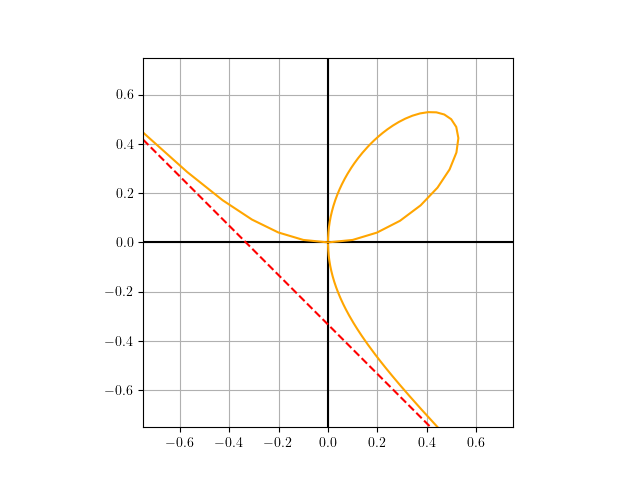
\includegraphics[width=0.5\textwidth, scale=1]{folium.png}
 \caption{Représentation graphique du folium de Descartes}
 \label{fig:folium}
\end{figure}

\emph{Remarque}~:
soit $\Psi : I \longmapsto \R$ continue et $\Gamma$ le graphe de $\Psi$. $\Gamma$ peut être considérée comme une courbe paramétrée $x(t)=t \quad y(t)=\Psi(t)$. On définit $\fonction{f}{I}{\R^2}{t}{(x(t),y(t))}$. Si $\Psi$ est dérivable alors pour tout réel $t$ de I on a $f'(t)=(1;\Psi'(t))$ alors tous les points sont réguliers. Si $\Psi$ est deux fois dérivable alors $f$ est deux fois dérivable et pour tout réel $t$ de I on a $f''(t)=(0,\Psi''(t))$, alors $\Det(f'(t),f''(t))=\Psi''(t)$ et donc l'équivalence est vraie
\begin{equation}
 t_0 \text{~est un point birégulier } \iff \Psi''(t_0) \neq 0.
\end{equation}

\section{Courbes en polaires}
Soient I un intervalle de $\R$, $r$ une application de I vers $\R$ au moins de classe $\classe{1}$. On considère la courbe définie par l'équation polaire $\rho=r(\theta)$, qu'on étudie comme un arc paramétré par $\theta$. On note $M(\theta)$ le point \og courant \fg{}.

\subsection{Étude locale en un point}
\subsubsection{Dérivation}
On sait que $\theta(t)=\theta \quad \theta'(t)=1 \quad \theta''(t)=0$ alors si $r$ et deux fois dérivable, en appliquant la formule de la section~\ref{subsec:not} on arrive à
\begin{align}
 \derived{\vect{OM}}{\theta}(\theta)&=r'(\theta) \vu_\theta + r(\theta) \vv_\theta;\\
 \deriveds{\vect{OM}}{\theta}(\theta)&=(r''(\theta)-r(\theta)) \vu_\theta + 2r'(\theta) \vv_\theta.
\end{align}

\subsubsection{Points réguliers}
Pour tout réel $\theta$ de I,
\begin{equation}
 \derived{\vect{OM}}{\theta}(\theta)=0 \iff
 \begin{cases}
   r'(\theta) = 0 \\ r(\theta)=0
 \end{cases}.
\end{equation}
Tous les points différents du pôle (ou origine) sont réguliers. En un point tel que $r(\theta) \neq 0$, la courbe \og tourne autour du pôle dans le sens direct \fg{}. Si le rapport $\frac{r'(\theta)}{r(\theta)}$ est négatif (resp.\ positif) alors $r(\theta)$ se rapproche (resp.\ s'éloigne) du pôle.

\subsubsection{Points d'annulation}
On suppose ici que $\theta_0$ est un zéro \emph{isolé} de la fonction $r$, c'est-à-dire $r(\theta_0)=0$ et il existe $\epsilon >0$ tel que pour tout réel $\theta$ de l'intervalle ouvert $\intervalleoo{\theta_0-\epsilon}{\theta_0+\epsilon}\setminus\{\theta_0\}$, on a $r(\theta) \neq 0$

\begin{prop}[admise]
 Soit $\theta_0$ un zéro isolé de la fonction $r$, alors $\Gamma$ admet pour tangente en $M(\theta_0)$ la droite $\Dr_{\theta_0}$. De plus~:
 \begin{enumerate}
 \item si $r$ change de signe en $\theta_0$ alors le point est d'allure normale (comme par exemple un cercle qui passe par le pôle);
 \item si $r$ s'annule sans changer de signe alors le point est un point de rebroussement de première espèce (comme par exemple une cardioïde).
 \end{enumerate}
\end{prop}

\subsection{Étude aux bornes}
\subsubsection{Lorsque $\theta$ tend vers l'infini}
Si la fonction $r$ tend vers zéro lorsque $\theta$ tend vers l'infini, alors le point courant tend vers le pôle. $\Gamma$ n'admet pas d'asymptote et on dit que le pôle est un \emph{point asymptote}.

Si la fonction $r$ tend vers un réel $a$ non nul lorsque $\theta$ tend vers l'infini, alors la distance du point courant au cercle $\cercle{0}{\abs{a}}$ tend vers zéro et donc c'est un \emph{cercle asymptote}.

Si par contre la fonction $r$ tend vers l'infini lorsque $\theta$ tend vers l'infini, alors la courbe admet une branche infinie sans direction asymptotique, on parle de \emph{branche spirale}.

\subsubsection{Lorsque $\theta$ tend vers $\theta_0$}
Si la fonction $r$ tend vers une limite finie, il n'y a rien de particulier. Par contre si la fonction $r$ tend vers l'infini lorsque $\theta$ tend vers $\theta_0$, alors la courbe admet une branche infinie de direction asymptotique $\vu_{\theta_0}$. On analyse s'il y a une asymptote. Pour le faire, on effectue un changement de repère et on se place dans le repère $\Rep'$ déduit du repère $\Rep$ par une rotation de centre $O$ et d'angle $\theta_0$. Les coordonnées cartésiennes de $M(\theta)$ dans $\Rep'$ seront alors
\begin{equation}
  M(\theta)
  \begin{cases}
    X(\theta)=r(\theta)\cos(\theta-\theta_0)\\
    Y(\theta)=r(\theta)\sin(\theta-\theta_0)
  \end{cases}.
\end{equation}
Lorsque $\theta$ tend vers $\theta_0$, $X(\theta)$ tend vers l'infini et $Y(\theta)$ est une forme indéterminée. Deux cas se présentent~:
\begin{itemize}
\item si $Y$ tend vers une limite finie $L$ alors la courbe admet une asymptote d'équation $y=L$ dans $\Rep'$;
\item sinon la courbe n'admet pas d'asymptote, le graphe présente une branche parabolique de direction asymptotique $\vu_{\theta_0}$.
\end{itemize}

\subsection{Symétries}
On cherche de nouveau à réduire l'intervalle d'étude. Une liste non-exhaustive de transformation est donnée dans la table~\ref{tab:sympol}.
\begin{table}
  \centering
  \begin{tabular}{|c|c|}\hline
    Hypothèse & Transformation \\ \hline
    $r(-\theta)=r(\theta)$ & Symétrie / $(Ox)$ \\ \hline
    $r(-\theta)=-r(\theta)$ & Symétrie / $(Oy)$ \\ \hline
    $r(\theta+\alpha)=kr(\theta)$ & Similitude directe de centre O \\ & d'angle $\alpha$ et de rapport k \\ \hline
    $r(\alpha-\theta)=r(\theta)$ & Symétrie / droite $\Dr_{\alpha/2}$ \\ \hline
    $r(\alpha-\theta)=-r(\theta)$ & Symétrie / droite $\Dr_{\pi/2 + \alpha/2}$ \\ \hline
 \end{tabular}
 \caption{Table des symétries}
 \label{tab:sympol}
\end{table}
Si la fonction $r$ est de période $T$, alors on peut réduire l'intervalle d'étude.
\subsection{Points multiples}\index{multiple}
Le point $M(\theta)$ est un point multiple si et seulement s'il existe $\theta' \neq \theta$ tel que $M(\theta)=M(\theta')$ c'est-à-dire si et seulement si
\begin{align}
 r(\theta)&=r(\theta')=0, \\
 r(\theta)&=r(\theta') \quad \congru{\theta}{\theta'}{2\pi},\\
 r(\theta)&=-r(\theta') \quad \congru{\theta}{\theta'+\pi}{2\pi}.
\end{align}
On se placera sur un intervalle, le plus petit possible, qui permet d'obtenir toute la courbe.
\subsection{Plan d'étude globale}
\begin{enumerate}
\item Ensemble de définition de la fonction $r$;
\item Restriction du domaine d'étude par la recherche de symétries et périodes;
\item Étude de $r$~: variations, signe, points d'annulation, tangentes remarquables;
\item Étude aux bornes;
\item Tracé de la courbe (le morceau étudié puis complétion par symétrie);
\item Éventuellement les points multiples.
\end{enumerate}

\subsection{Exemple}

Soit $\Gamma$ définie par $r(\theta)=\cos \theta + \cos 3\theta$. La fonction $r$ est définie sur $\R$ tout entier. Elle est $2\pi$-périodique, on peut donc restreindre l'étude à $\intervalleff{-\pi}{\pi}$. Puisque la fonction cosinus est paire, la fonction $r$ est aussi paire, on peut donc encore restreindre le domaine d'étude à $\intervalleff{0}{\pi}$ et ensuite on complétera la courbe par une symétrie d'axe $(Ox)$. Pour tout réel $\theta \in \intervalleff{0}{\pi}$ on a $r(\pi-\theta)=-r(\theta)$ alors on peut restreindre l'étude sur $\intervalleff{0}{\frac{\pi}{2}}$ puis on complète par une symétrie d'axe $\Dr_{\pi/2+\pi/2}$ c'est-à-dire $(Ox)$. On fait deux fois la même symétrie, cela signifie qu'on obtient toute la courbe pour $\theta \in \intervalleff{0}{\pi}$. Au final le domaine d'étude est restreint à $\intervalleff{0}{\frac{\pi}{2}}$

Soit $\theta \in \intervalleff{0}{\frac{\pi}{2}}$, alors $r(\theta)=\cos \theta + \cos 3\theta=2\cos(2\theta)\cos \theta$ d'après les transformations produit en somme. Donc
\begin{equation}
  r(\theta)=0 \iff \cos(2\theta)=0 \text{~ou~} \cos \theta=0 \iff \theta \in \left\{\frac{\pi}{4}; \frac{\pi}{2}\right\}.
\end{equation}
La fonction $r$ est dérivable sur $\intervalleff{0}{\frac{\pi}{2}}$. Pour tout $\theta \in \intervalleff{0}{\frac{\pi}{2}}$, on a
\begin{equation}
 r'(\theta)=-\sin\theta - 3 \sin(3 \theta).
\end{equation}
De plus on sait que $\sin(3 \theta) = \Im(\e^{\ii 3\theta})$ et
\begin{equation}
 \e^{\ii 3 \theta}=\cos^3 \theta + 3\cos^2 \theta \ii \sin \theta + 3 \cos \theta \ii^2 \sin^2 \theta + \ii^3\sin^3 \theta.
\end{equation}
 Ainsi $\sin(3 \theta) = 3 \sin\theta \cos^2 \theta - \sin^3 \theta$. En introduisant $\sin^2=1-\cos^2$ dans l'équation et en factorisant, on arrive à
 \begin{equation}
  r'(\theta)=2 \sin \theta (1-6 \cos^2 \theta).
 \end{equation}
Alors
\begin{equation}
 r'(\theta)=0 \iff \sin\theta=0 \text{~ou~} \cos^2 \theta = \frac{1}{6} \iff \theta \in \left\{0, \arccos\left(\frac{1}{\sqrt{6}}\right)\right\}.
\end{equation}
\begin{itemize}
\item En $\frac{\pi}{4}$, on a $r\left(\frac{\pi}{4}\right)=0$ et $r'\left(\frac{\pi}{4}\right)=-2\sqrt{2}$ et donc $\derived{\vec{M}}{\theta}\left(\frac{\pi}{4}\right) = -2\sqrt{2}\vec{u}_{\frac{\pi}{4}}$ La tangente est donc la première bissectrice;
\item en $\theta_0=\arccos\left(\frac{1}{\sqrt{6}}\right)$, on a $r'(\theta_0)=0$ et
 \begin{align}
  r(\theta_0) & = \cos(\theta_0) + \cos(3 \theta_0) \\
  & = \frac{1}{\sqrt{6}} + \cos^3\theta_0 - 3 \sin^2\theta_0 \cos\theta_0 \\
  & = \frac{\sqrt{6}}{6} \left(1+\frac{1}{6}-3\left(1-\frac{1}{6}\right)\right) \\
  & = -\frac{2\sqrt{6}}{9}
 \end{align}
En $\theta_0$, la tangente est perpendiculaire à $(OM(\theta_0))$.
\end{itemize}
\begin{itemize}
\item En $0$, $r'(0)=0$ et $r(0)=2$ et donc $\derived{\vec{M}}{\theta}(0)=2 \vec{v}_0=2 \vj$, la tangente est parallèle à $(Oy)$;
\item En $\frac{\pi}{2}$, $r\left(\frac{\pi}{2}\right)=0$ et $r'\left(\frac{\pi}{2}\right)=2$ et donc $\derived{\vec{M}}{\theta}\left(\frac{\pi}{2}\right)=2 \vec{v}_0=2 \vj$, la tangente est parallèle à $(Oy)$.
\end{itemize}
On trace cette courbe paramétrée sur la figure~\ref{fig:pol}.
\begin{figure}
 \centering
 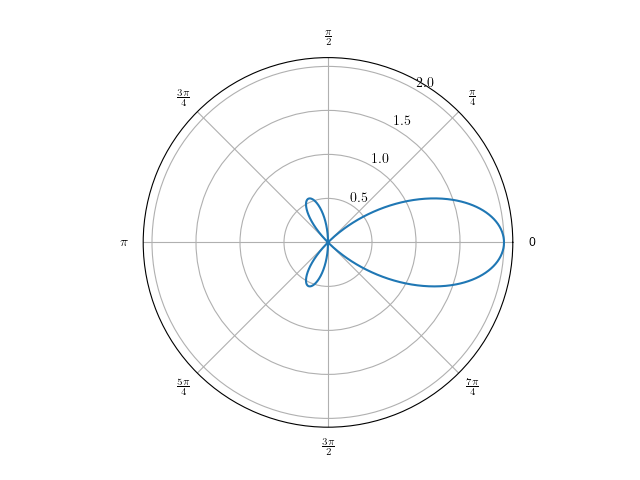
\includegraphics[width=0.5\textwidth,scale=1]{courbepolaire.png}
 \caption{Courbe polaire définie par $r(\theta)=\cos\theta+\cos(3\theta)$}
 \label{fig:pol}
\end{figure}
